



\section{Explanations}
\label{sec:appendix-shapleys}


\iffalse
\begin{figure}[h]
% \vspace{1mm}
% \begin{center}
%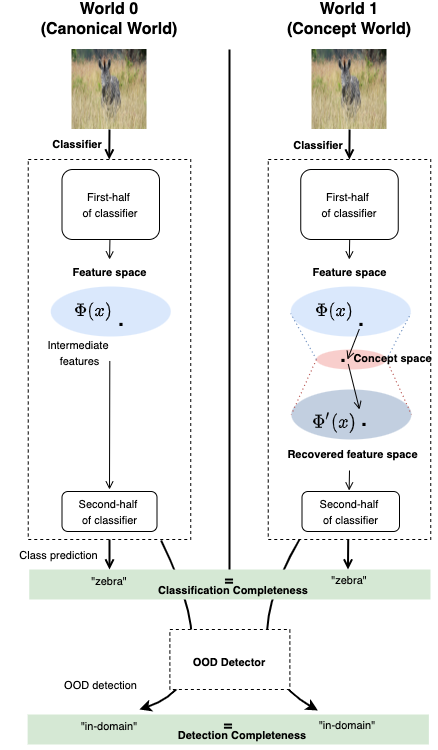
\includegraphics[width=0.45\textwidth]{figures/completeness.png}
% \hspace*{+.5cm} 
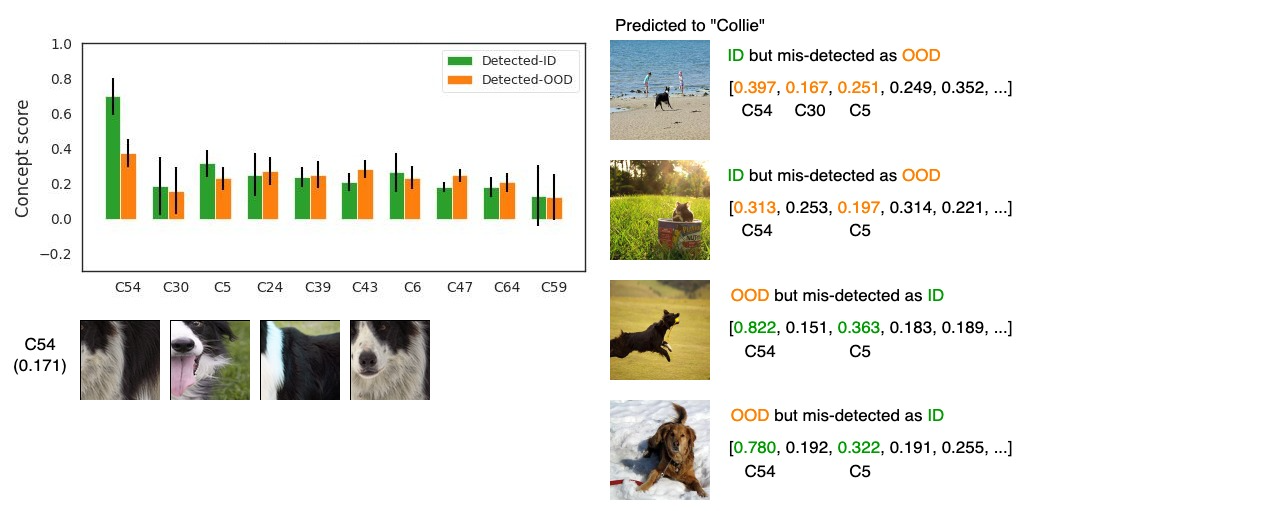
\includegraphics[scale=0.35]{figures/expl_collie.png}
% \vspace{-9mm}
\caption{
\small \textbf{Our concept-based explanations for Energy detector}~\citep{liu2020energy}. Concepts are discovered by our method with $\lambda_\textrm{mse} = 1, \lambda_\textrm{norm} = 0.1, \lambda_\textrm{sep} = 10$.}
\label{fig:expl_collie}
% \end{center}
\end{figure}
\fi

\subsection{Important Concepts for Each OOD Detector}
\label{sec:appendix-explanation}
We show additional examples for the top-ranked concepts by $\textrm{SHAP}(\eta_{\bff, S}, \bfc_i)$ in Fig. \ref{fig:app-shap}.
For each figure with a fixed choice of class prediction, we present receptive fields from ID test set corresponding to top concepts that contribute the most to the decisions of each OOD detector.
All receptive fields passed the threshold test that the inner product between the feature representation and the corresponding concept vector is over $0.85$.
\begin{figure*}[ht]
\centering
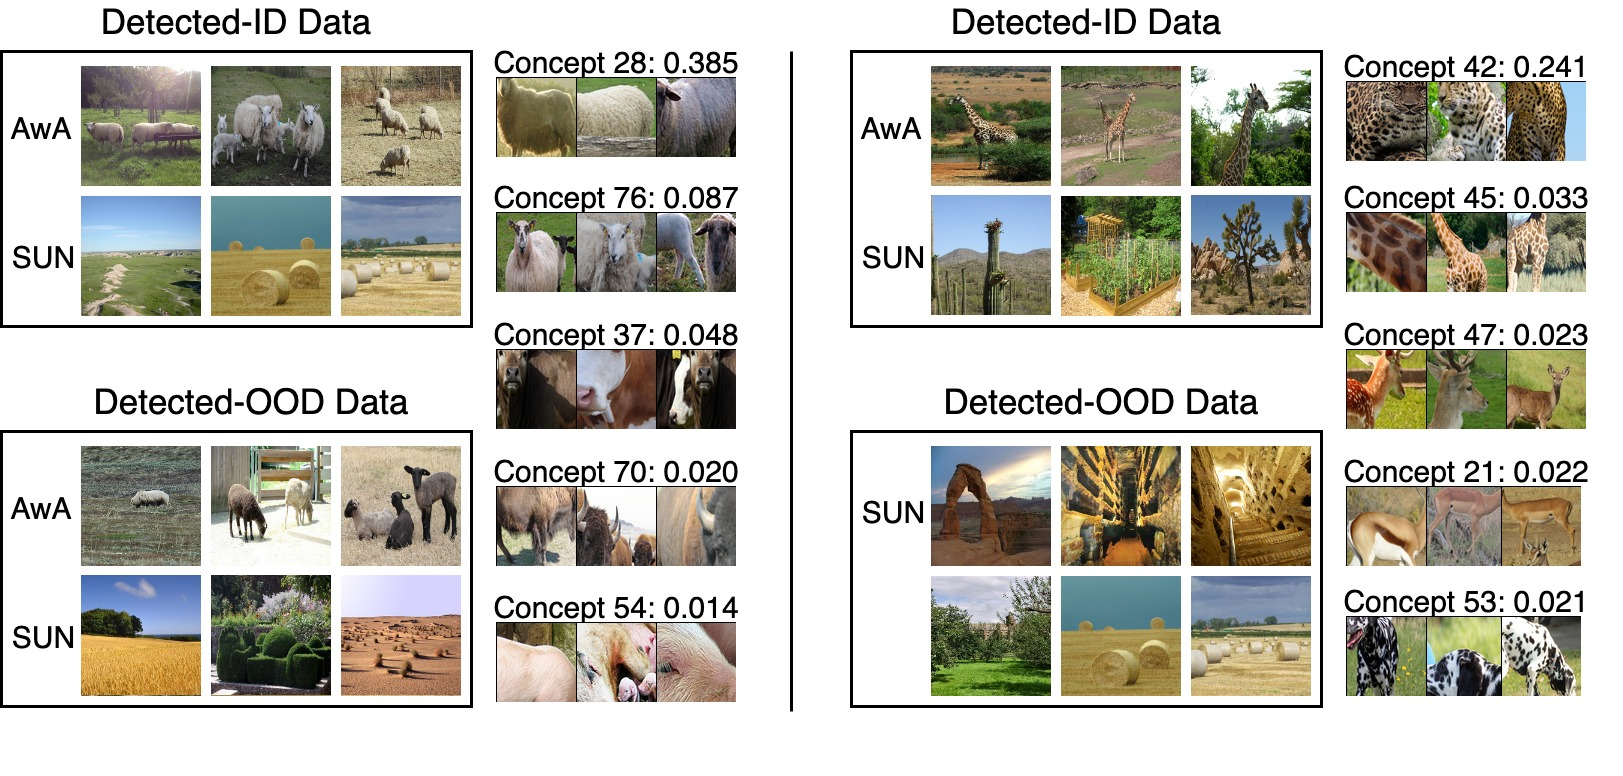
\includegraphics[width=\textwidth]{figures/concepts.jpg}
\vspace{-0.3in}
\caption{Top-6 important concepts for the Energy OOD detector with respect to class ``Sheep'' (on the left) and class ``Giraffe'' (on the right).}
\label{fig:app-shap}
\end{figure*}

Moreover, in Fig. \ref{fig:shap_buffalo}, we compare the important concepts discovered by the baseline method \cite{yeh2020completeness} (denoted as ``baseline'') vs. ours.
With the baseline, when the learned concepts are solely intended for reconstructing the behavior of the classifier, we observe that interpretation of both the classifier and OOD detector depends on a common set of concepts (\ie concepts 32, 10, and 47).
On the other hand, the concepts learned by our method focus on reconstructing the behavior of both the OOD detector and the classifier. In this case, we observe that a distinct set of important concepts are selected for classification and OOD detection.
We also observe that our method requires more concepts in order to address the decisions of both the classifier and OOD detector.
For instance, the number of concepts obtained by our method and the baseline are 78 and 53 (respectively), out of a total 100 concepts after the duplicate removal of concept vectors.
In short, when the concepts are only targeted at explaining the DNN classifier (as in the baseline \cite{yeh2020completeness}), the behavior of the OOD detector is merely described by the common set of concepts that are important for the DNN classifier.
On the other hand, when not only the DNN classifier but also the OOD detector is taken into consideration during concept learning (\ie our method), we obtain a more diverse and expanded set of concepts, and different concepts play a major role in interpreting the classification and detection results. 

\begin{figure}[hbt]
% \vspace{1mm}
\centering
%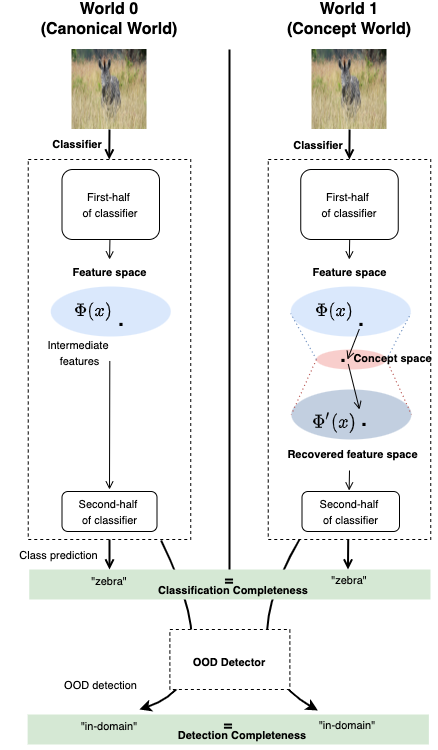
\includegraphics[width=0.45\textwidth]{figures/completeness.png}
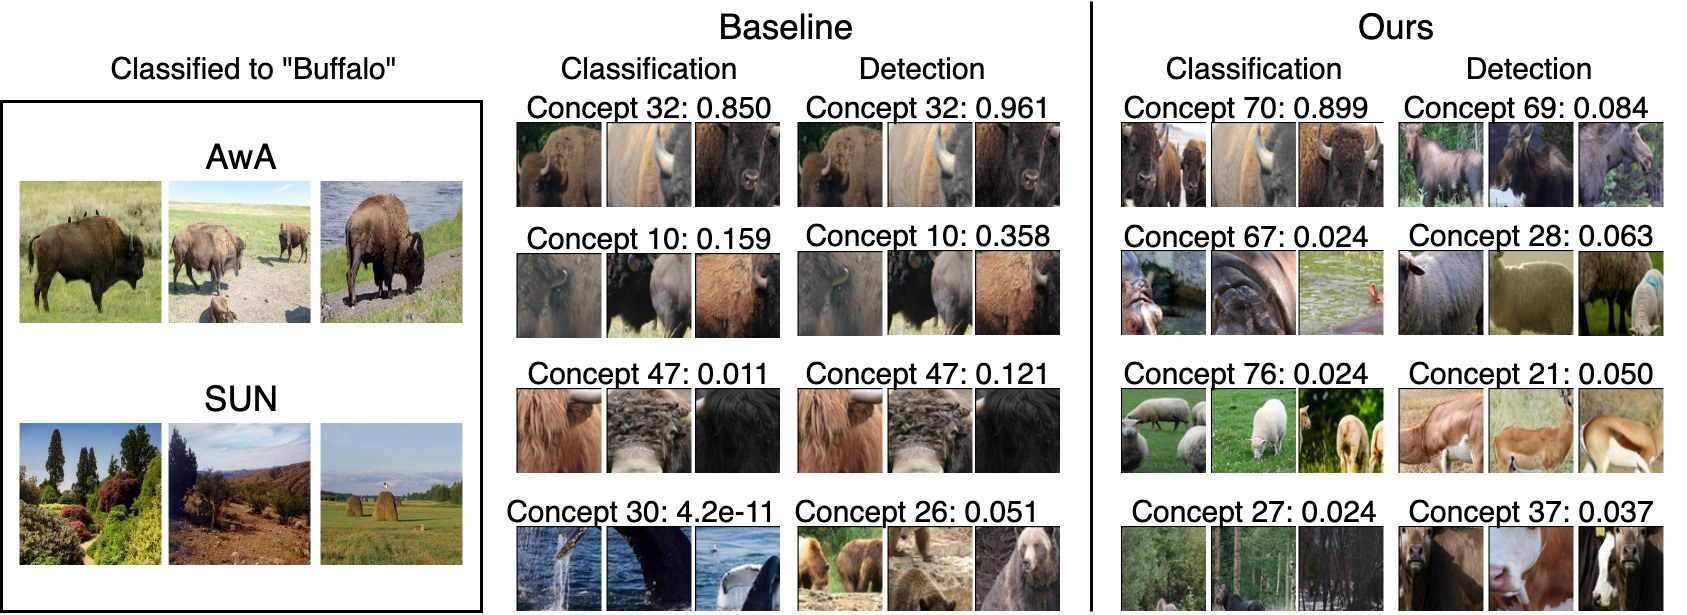
\includegraphics[width=\textwidth]{figures/expl_buffalo.jpeg}
% \vspace{-9mm}
\caption{\textbf{Most important concepts for the Energy detector with respect to the predicted class ``Buffalo''.} 
% Concepts are obtained by our concept learning algorithm with $\lambda_\textrm{mse} = 1, \lambda_\textrm{norm} = 0.1, \lambda_\textrm{sep} = 0$.
We demonstrate randomly sampled images that are predicted by the classifier into this class. 
We compare the top-4 important concepts to describe the DNN classifier (and Energy detector), ranked by the Shapley value based on classification completeness $\textrm{SHAP}(\eta^{j}_{\bff}, \bfc_i)$ (and detection completeness $\textrm{SHAP}(\eta^{j}_{\bff, S}, \bfc_i)$).
``Baseline'' corresponds to the case when the concepts are learned with $\lambda_\textrm{mse} = \lambda_\textrm{norm} = \lambda_\textrm{sep} = 0$, whereas ``Ours'' corresponds to the concepts learned with $\lambda_\textrm{mse} = 1, \lambda_\textrm{norm} = 0.1, \lambda_\textrm{sep} = 0$.
% To visualize what each concept represents, we display the top receptive fields from $\Dinte$ whose inner-product with the corresponding concept vector is larger than 0.8.
}
% \vspace{-5mm}
\label{fig:shap_buffalo}
\end{figure}

\subsection{More Examples of Our Concept-Based Explanation}
\label{app:more-expl}
In Fig.~\ref{fig:expl-additional1}, we provide additional examples of the concept-based explanations provided by  our method and compare it with that of \cite{yeh2020completeness}.

% \textcolor{blue}{Needs a couple of lines about the takeaway message.}



\begin{figure*}[b]
  \centering
  \begin{subfigure}{\linewidth}
    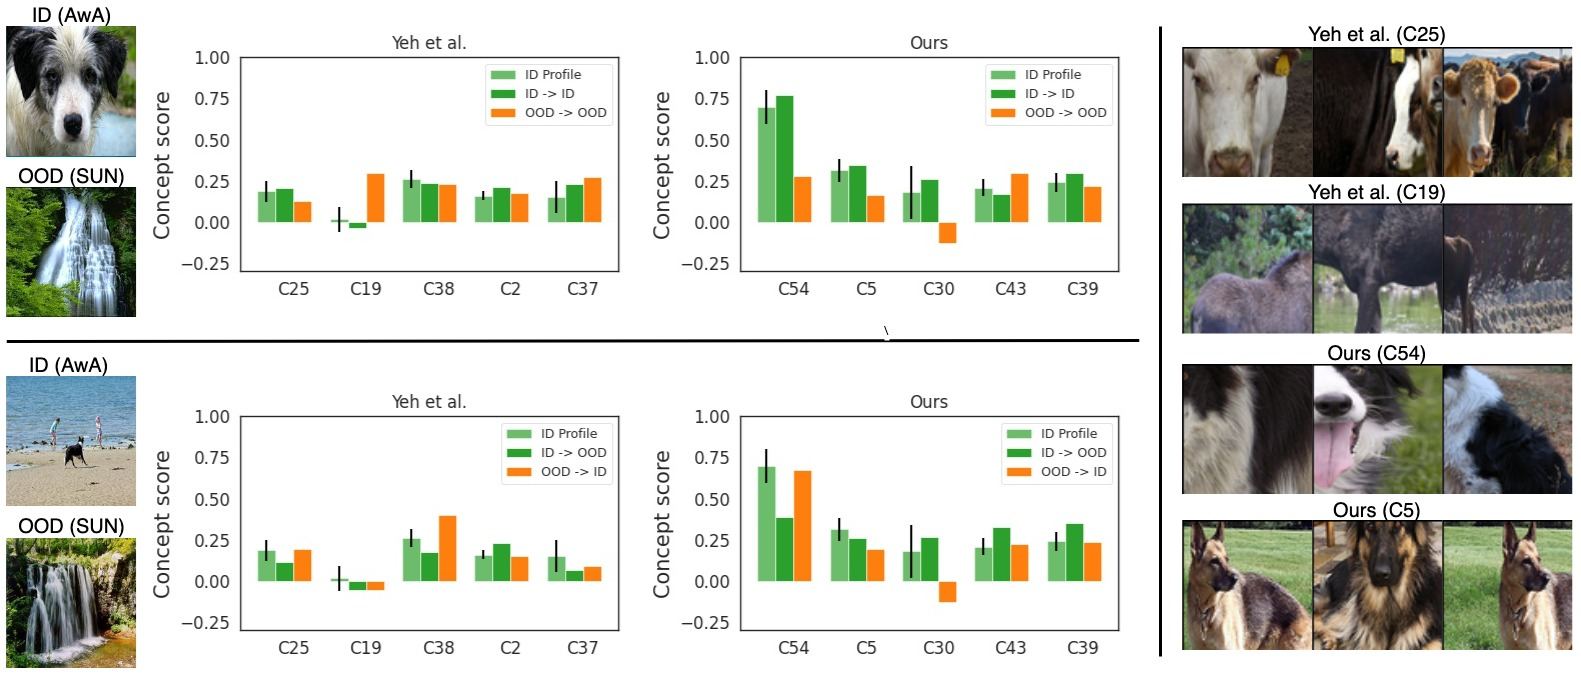
\includegraphics[width=\textwidth]{figures/energy_SUN_Collie.jpg}
    \caption{class ``Collie'', Energy OOD detector. Images randomly selected from AwA test set and \texttt{SUN}.}
    % \label{fig:expl-energy-collie}
  \end{subfigure}
  \\
  \begin{subfigure}{\linewidth}
    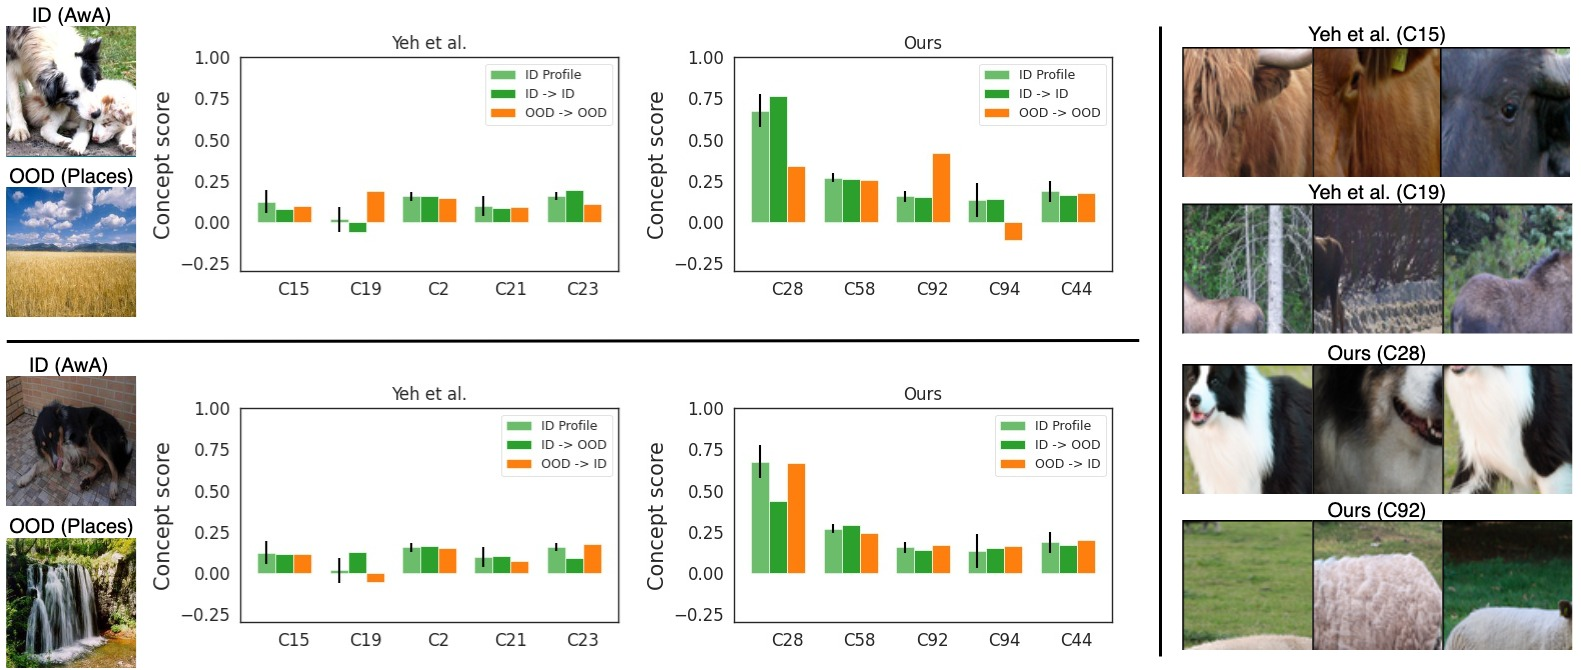
\includegraphics[width=\textwidth]{figures/MSP_SUN_Collie.jpg}
    \caption{class ``Collie'', MSP OOD detector. Images randomly selected from AwA test set and \texttt{SUN}.}
    % \label{fig:expl-energy-collie}
  \end{subfigure}
  % \vspace{.1in}
  % \caption{\textcolor{blue}{\textbf{Concept-based explanations using concepts by Yeh et al. vs. ours.} 
    % ID profile shows the concept-score patterns for normal ID images.}}
\label{fig:expl-additional}
\end{figure*}
  
\begin{figure*}\ContinuedFloat
  \centering
  \begin{subfigure}{\linewidth}
    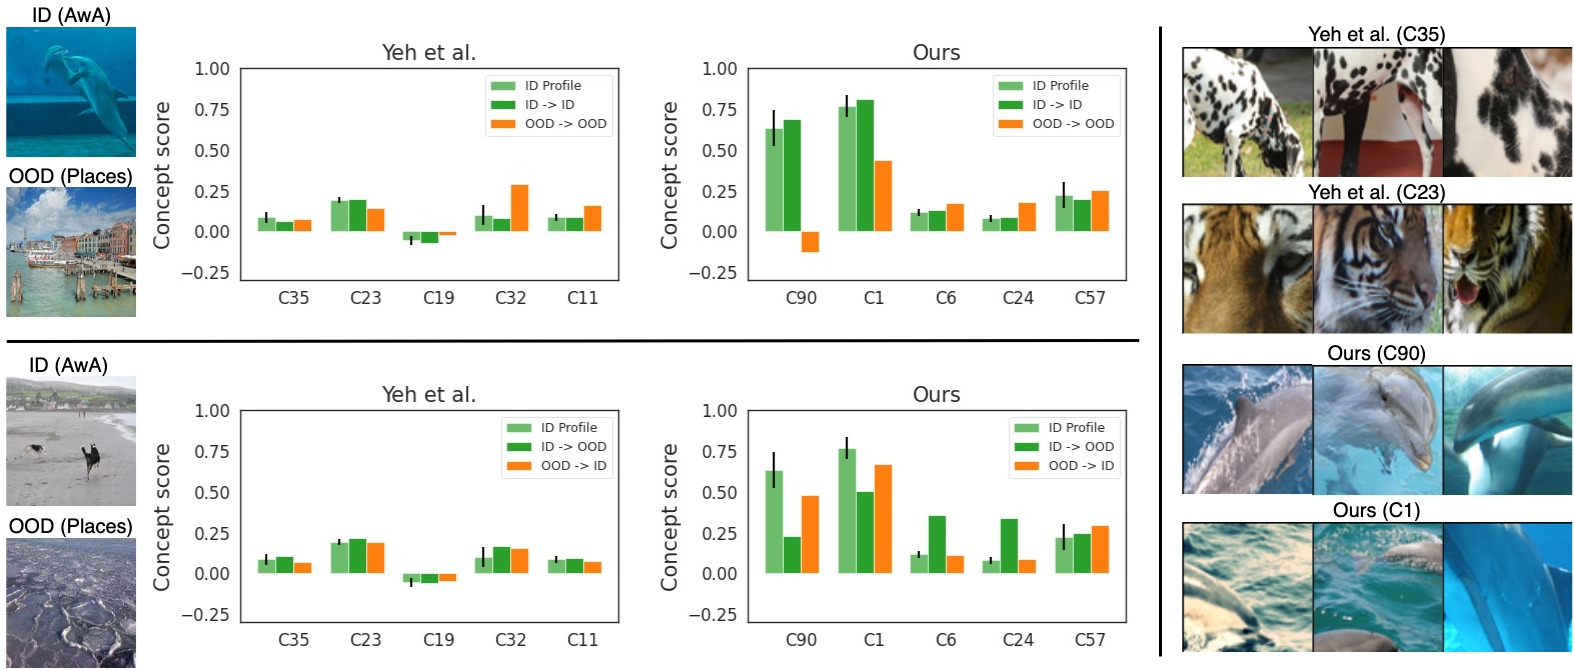
\includegraphics[width=\textwidth]{figures/energy-dolphin.jpg}
    \caption{class ``Dolphin'', Energy OOD detector. Images randomly selected from AwA test set and \texttt{Places}.}
    \label{fig:expl-energy-dolphin}
  \end{subfigure}
  \\
  \begin{subfigure}{\linewidth}
    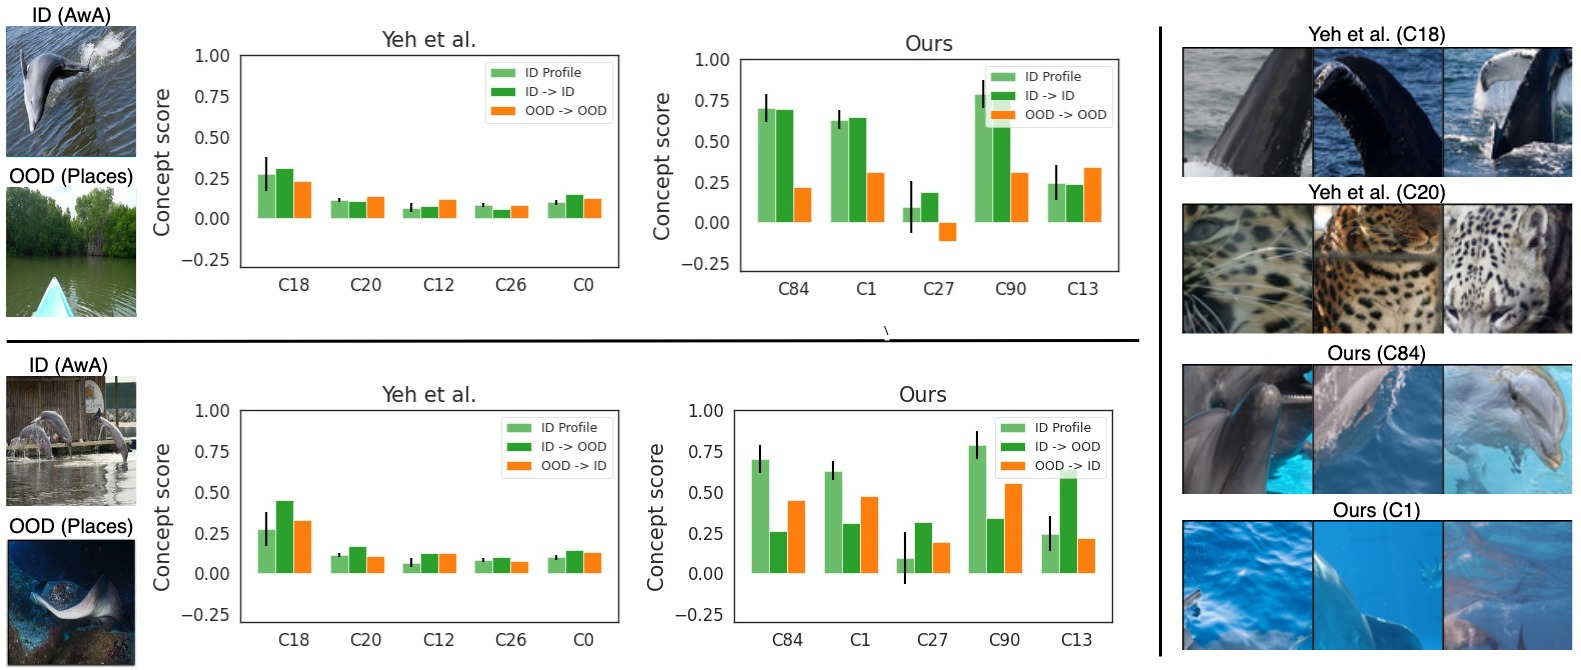
\includegraphics[width=\textwidth]{figures/MSP_Places_Dolphin.jpg}
    \caption{class ``Dolphin'', MSP OOD detector. Images randomly selected from AwA test set and \texttt{Places}.}
    \label{fig:expl-msp-dolphin}
  \end{subfigure}
  \vspace{.1in}
  \caption{\textbf{Concept-based explanations using concepts identified by \citet{yeh2020completeness} vs. ours.}
ID profile shows the average concept-score pattern for normal ID images.}
\label{fig:expl-additional1}
\end{figure*}

\iffalse
\newpage
\subsection{Counterfactual Analysis}
\label{sec:appendix-counterfactual}
% To further verify the contribution of concepts quantified by Eqn. (\ref{equ: ConceptSHAP}), we conduct counterfactual analysis, addressing the following questions: \textit{if the input had these concepts as a dominant features, would it have been detected as ID (or OOD)?}

%
\begin{wrapfigure}{r}{0.5\linewidth}
% \begin{figure}[t]
% \vspace{-10mm}
\centering
%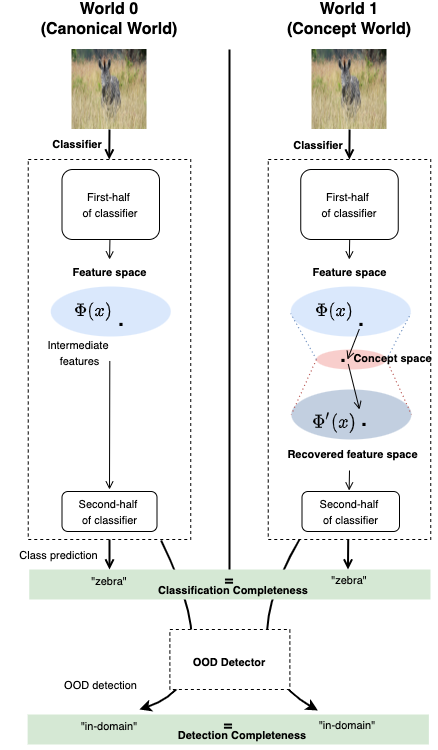
\includegraphics[width=0.45\textwidth]{figures/completeness.png}
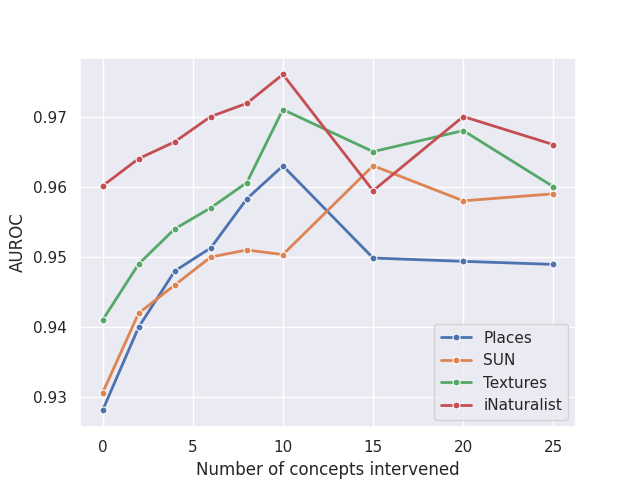
\includegraphics[scale=0.4]{figures/intervention_msp.png}
%\vspace{-2mm}
\caption{Performance of MSP with test-time interventions on concept scoress.}
% \vspace{-5mm}
\label{fig:intervention_msp}
\end{wrapfigure}
% \end{figure}
To verify the important concepts identified by our modified Shapley value, we perform counterfactual analysis, addressing the following question: \textit{if the OOD detector thought the input has different score for this concept, would the detection result be different?}
As we do not assume to have groundtruth annotation for concepts, we construct concept score profiles of detected-ID (or detected-OOD) inputs from held-out ID (or OOD) dataset, and refer to this as ID (or OOD) concept profile.
With the guidance of ID and OOD concept profiles, we take intervention on the concept scores of mis-detected inputs.
Specifically, for ID data mis-detected as OOD, we update their concept scores using ID profiles, and similarlly, for OOD data mis-detected as ID, their concept scores are updated with OOD profiles.
The number of concepts to be intervened can be varied.
As shown in Figure \ref{fig:intervention_msp}, with intervention on more number of important concepts (ranked by $\textrm{SHAP}(\eta^{}_{\bff, S}, \bfc_i)$)), we observe an improved performance of OOD detector in concept world.
\fi